\documentclass[a4paper,14pt,oneside,openany]{memoir}

\usepackage[left=30mm, right=15mm, top=20mm, bottom=20mm]{geometry}
\pagestyle{plain}
\parindent=1.25cm
\usepackage{indentfirst}

\usepackage{fontspec}
\usepackage[english, russian]{babel}

\setmainfont{LiberationSerif}[
    Path = fonts/,
    Extension = .ttf,
    UprightFont = *-Regular,
    BoldFont = *-Bold,
    ItalicFont = *-Italic,
    BoldItalicFont = *-BoldItalic
]

\setmonofont{LiberationMono}[
    Path = fonts/,
    Extension = .ttf,
    UprightFont = *-Regular,
    BoldFont = *-Bold,
    ItalicFont = *-Italic,
    BoldItalicFont = *-BoldItalic
]

\setsecnumdepth{subsection}
\renewcommand*{\chapterheadstart}{}
\renewcommand*{\printchaptername}{}
\renewcommand*{\chapnumfont}{\normalfont\bfseries\large}
\renewcommand*{\afterchapternum}{\hspace{1em}}
\renewcommand*{\printchaptertitle}{\normalfont\bfseries\large\centering}
\setbeforesecskip{18pt}
\setaftersecskip{14pt}
\setsecheadstyle{\raggedright\normalfont\bfseries\normalsize}
\setbeforesubsecskip{14pt}
\setaftersubsecskip{10pt}
\setsubsecheadstyle{\raggedright\normalfont\bfseries\small}
\setbeforesubsubsecskip{12pt}
\setaftersubsubsecskip{8pt}
\setsubsubsecheadstyle{\raggedright\normalfont\bfseries\small}

\addto\captionsrussian{\renewcommand\contentsname{Содержание}}
\setrmarg{2.55em plus1fil}
\renewcommand{\aftertoctitle}{\afterchaptertitle \vspace{-\cftbeforechapterskip}}
\renewcommand*{\cftchapternumwidth}{1.5em}
\renewcommand*{\cftchapterfont}{\normalfont}
\renewcommand*{\cftchapterpagefont}{\normalfont}
\renewcommand*{\cftchapterdotsep}{\cftdotsep}
\renewcommand*{\cftdotsep}{1}
\renewcommand*{\cftchapterleader}{\cftdotfill{\cftchapterdotsep}}
\maxtocdepth{subsection}

\tolerance 1414
\hbadness 1414
\emergencystretch 1.5em
\hfuzz 0.3pt
\vfuzz \hfuzz
\clubpenalty=10000
\widowpenalty=10000
\brokenpenalty=4991
\sloppy

\usepackage{graphicx}
\usepackage{caption}
\usepackage{float}
\usepackage{enumitem}
\usepackage{array}
\usepackage{longtable}
\usepackage{booktabs}
\usepackage{listings}
\usepackage{hyperref}
\usepackage{amsmath,amssymb}

\graphicspath{{images/}}
\captionsetup[figure]{font=small, width=\textwidth, name=Рисунок, justification=centering}
\captionsetup[table]{singlelinecheck=false,font=small,width=\textwidth,justification=justified}
\captiondelim{. }
\setkeys{Gin}{width=\textwidth}
\counterwithout{figure}{chapter}
\counterwithout{table}{chapter}
\setlist{noitemsep, leftmargin=*}
\hypersetup{colorlinks=true, linkcolor=black, urlcolor=blue}
\renewcommand\UrlFont{\footnotesize\ttfamily}
\lstset{
    basicstyle=\ttfamily\small,
    breaklines=true,
    columns=fullflexible,
    frame=single,
    keepspaces=true,
    showstringspaces=false
}

\begin{document}

\thispagestyle{empty}

\begin{center}
    МИНИСТЕРСТВО ЦИФРОВОГО РАЗВИТИЯ, СВЯЗИ И МАССОВЫХ \\
    КОММУНИКАЦИЙ РОССИЙСКОЙ ФЕДЕРАЦИИ

    \vspace{16pt}

    Федеральное государственное бюджетное образовательное учреждение \\
    высшего образования \\
    «Сибирский государственный университет телекоммуникаций \\
    и информатики» (СибГУТИ)

    \vspace{16pt}

    Кафедра прикладной математики и кибернетики \\
    (ПМ и К)
\end{center}

\vfill

\begin{center}
    Отчёт \\
    по лабораторной работе №~5 \\
    «Нейронные сети для обработки изображений»
\end{center}

\vfill

\noindent Выполнили: \\
\noindent\begin{tabular*}{\textwidth}{@{}l@{\extracolsep{\fill}}r@{}}
\textit{студенты группы ИП-414} & \textit{М.~Р.~Зинаков} \\
& \textit{А.~А.~Карев}
\end{tabular*}

\vspace{16pt}

\noindent Работу проверил: \\
\noindent\begin{tabular*}{\textwidth}{@{}l@{\extracolsep{\fill}}r@{}}
\textit{старший преподаватель каф. ПМ и К} & \textit{К.~И.~Дементьева}
\end{tabular*}

\vfill

\begin{center}
    Новосибирск 2026 г.
\end{center}


\newpage
\setcounter{page}{2}
\OnehalfSpacing*

\tableofcontents*

\chapter*{Введение}
\addcontentsline{toc}{chapter}{Введение}

\textbf{Цель работы:} освоить на практике принципы построения, обучения и комплексной оценки сверточных нейронных сетей (Convolutional Neural Networks, CNN) для решения базовых прикладных задач компьютерного зрения, исследовать влияние слоев пакетной нормализации (BatchNormalization) и параметров стохастического градиентного спуска (SGD) на сходимость оптимизационного процесса и обобщающую способность модели.

В соответствии с методическими указаниями к лабораторной работе №~5 кафедры Прикладной математики и кибернетики СибГУТИ, распределение индивидуального задания определяется номером студента в журнале группы: $N_{\text{сп}} = 9$.

\textbf{Параметры индивидуального варианта:}
\begin{enumerate}
    \item \textit{Выбор набора данных:}
    \begin{equation*}
        N_{\text{датасет}} = (N_{\text{сп}} \bmod 6) + 1 = (9 \bmod 6) + 1 = 4 \implies \textbf{Oxford Flowers 102}.
    \end{equation*}
    Коллекция Oxford Flowers 102 содержит 8189 изображений цветковых растений, сгруппированных по 102 классам (от 40 до 258 изображений на категорию). Выборка канонически разделена на обучающую (1020 кадров, строго по 10 примеров на класс), валидационную (1020 кадров) и генеральную тестовую (6149 кадров, более 75\,\% всего объема).
    \item \textit{Выбор архитектуры нейронной сети и оптимизатора:}
    \begin{equation*}
        N_{\text{архитектура}} = (N_{\text{сп}} \bmod 8) + 1 = (9 \bmod 8) + 1 = 2 \implies \textbf{Вариант 2}.
    \end{equation*}
    \begin{itemize}
        \item \textbf{Архитектура CNN:} 3 сверточных слоя (Conv2D) + 2 полносвязных слоя (Dense);
        \item \textbf{Регуляризация:} пакетная нормализация (BatchNormalization);
        \item \textbf{Оптимизатор:} стохастический градиентный спуск (SGD) с коэффициентом момента.
    \end{itemize}
\end{enumerate}

\textbf{Основные шаги выполнения работы:}
\begin{enumerate}
    \item \textbf{Шаг 1. Загрузка и подготовка данных:} исследование структуры выборки Oxford Flowers 102, визуализация репрезентативных категорий, масштабирование изображений к размеру $96 \times 96 \times 3$, нормализация интенсивностей каналов и построение конвейера данных \texttt{tf.data} с потоковой аугментацией.
    \item \textbf{Шаг 2. Создание архитектуры нейронной сети:} проектирование сверточной сети строго по Варианту 2 (3 сверточных блока с фильтрами 32, 64, 128, пакетной нормализацией BatchNormalization, нелинейностями ReLU и пулингом MaxPooling2D, объединенных с 2 полносвязными слоями на 256 и 102 нейрона) и компиляция с оптимизатором SGD.
    \item \textbf{Шаг 3. Обучение, анализ графиков и оценка точности:} обучение модели на 12 эпохах, анализ кривых сходимости функций потерь и метрик точности (Top-1 и Top-5), финальная оценка качества на генеральной тестовой выборке из 6149 изображений, сравнение с уровнем случайного угадывания и качественный анализ предсказаний.
\end{enumerate}

\vspace{12pt}
\noindent \textbf{Ссылка на интерактивный блокнот в Google Colab:} \\
{\footnotesize\url{https://colab.research.google.com/github/MichaelRayven/Machine-Learning-Algorithms/blob/feat/lab5/src/lab5/lab5.ipynb}}

\vspace{6pt}
\noindent \textbf{Репозиторий проекта на GitHub:} \\
{\footnotesize\url{https://github.com/MichaelRayven/Machine-Learning-Algorithms/tree/feat/lab5}}

\chapter{Теоретические основы сверточных нейронных сетей}

\section{Математическая модель двумерной дискретной свертки}

Классические полносвязные нейронные сети (Multi-Layer Perceptron, MLP) при обработке визуальных данных сталкиваются с проблемой экспоненциального роста числа обучаемых параметров и разрушения двумерной пространственной топологии изображения. Вытягивание матрицы пикселей в одномерный вектор утрачивает информацию о взаимном расположении соседних точек.

Сверточные нейронные сети (Convolutional Neural Networks, CNN) преодолевают указанное ограничение за счет двух ключевых архитектурных принципов: \textit{локальности рецептивных полей} и \textit{разделения весов} (weight sharing).

Операция двумерной дискретной свертки входной матрицы изображения $I \in \mathbb{R}^{H \times W}$ с обучаемым ядром (фильтром) $K \in \mathbb{R}^{k_h \times k_w}$ определяется выражением:
\begin{equation}
    S(i, j) = (I * K)(i, j) = \sum_{m=0}^{k_h - 1} \sum_{n=0}^{k_w - 1} I(i + m, j + n) K(m, n) + b,
    \label{eq:convolution}
\end{equation}
где $b \in \mathbb{R}$ --- смещение (bias), $S(i, j)$ --- результирующее значение в карте признаков (feature map).

При наличии $C_{\text{in}}$ входных каналов (для цветного RGB-изображения $C_{\text{in}} = 3$) и набора из $C_{\text{out}}$ фильтров, сверточный слой преобразует тензор размера $(H, W, C_{\text{in}})$ в тензор $(H', W', C_{\text{out}})$. Каждое ядро специализируется на выявлении определенных локальных паттернов: границы, градиенты яркости на первых слоях, текстуры и геометрические формы на промежуточных, целостные структуры лепестков и соцветий на глубоких уровнях абстракции.

После операции свертки к каждому элементу карты признаков применяется поэлементная нелинейная функция активации. В данной работе используется выпрямленная линейная единица $\text{ReLU}$ (Rectified Linear Unit):
\begin{equation}
    f(x) = \max(0, x),
    \label{eq:relu}
\end{equation}
производная которой равна единице при $x > 0$ и нулю при $x \le 0$. Данная функция исключает эффект насыщения и затухания градиентов, характерный для сигмоиды и гиперболического тангенса.

Для снижения размерности карт признаков и формирования инвариантности к малым геометрическим сдвигам применяется операция максимального объединения (MaxPooling):
\begin{equation}
    P(i, j) = \max_{0 \le m < p, \, 0 \le n < p} S(i \cdot s + m, \, j \cdot s + n),
    \label{eq:maxpool}
\end{equation}
где $p \times p$ --- размер окна пулинга (в работе $2 \times 2$), $s$ --- шаг (stride, $s = 2$). Пулинг сокращает пространственное разрешение в два раза по каждому измерению, уменьшая вычислительную сложность последующих слоев.

\section{Механизм пакетной нормализации (BatchNormalization)}

При последовательном прохождении сигнала через глубокие слои нейросети распределение входов каждого слоя непрерывно изменяется по мере обновления весов предыдущих слоев. Данный феномен известен как \textit{внутренний ковариационный сдвиг} (Internal Covariate Shift). Слоям приходится адаптироваться к изменяющимся масштабам и смещениям, что вынуждает использовать предельно малые скорости обучения и замедляет сходимость.

Слой пакетной нормализации (BatchNormalization, предложенный С.~Иоффе и К.~Сегеди) стабилизирует процесс оптимизации. Для каждого мини-батча $\mathcal{B} = \{x_1, x_2, \dots, x_m\}$ размера $m$ вычисляются выборочные среднее и дисперсия:
\begin{equation}
    \mu_\mathcal{B} = \frac{1}{m} \sum_{i=1}^m x_i, \qquad \sigma_\mathcal{B}^2 = \frac{1}{m} \sum_{i=1}^m (x_i - \mu_\mathcal{B})^2.
    \label{eq:bn_mean_var}
\end{equation}

Далее выполняется нормирование с добавлением малой константы $\epsilon = 10^{-3}$ для предотвращения деления на ноль:
\begin{equation}
    \hat{x}_i = \frac{x_i - \mu_\mathcal{B}}{\sqrt{\sigma_\mathcal{B}^2 + \epsilon}}.
    \label{eq:bn_norm}
\end{equation}

Для сохранения выразительной способности сети вводятся два обучаемых параметра --- масштаб $\gamma$ и сдвиг $\beta$:
\begin{equation}
    y_i = \gamma \hat{x}_i + \beta.
    \label{eq:bn_scale_shift}
\end{equation}

В сверточных слоях нормализация производится по пространственным осям и мини-батчу одновременно, сохраняя единые масштабирующие коэффициенты для каждой карты признаков. На этапе инференса используются накопленные экспоненциальные скользящие средние (moving averages), что обеспечивает детерминированность вычислений.

Пакетная нормализация выполняет две важнейшие функции:
\begin{enumerate}
    \item \textbf{Сглаживание ландшафта оптимизации:} функция потерь становится более липшицевой, градиенты не взрываются и не затухают, позволяя безопасно повышать скорость обучения.
    \item \textbf{Слабая регуляризация:} стохастические флуктуации статистик по мини-батчам вносят полезный шум, препятствующий сонастройке весов и снижающий эффект переобучения без необходимости принудительного обнуления нейронов, как в Dropout.
\end{enumerate}

\section{Оптимизация стохастическим градиентным спуском с моментом}

Стандартный градиентный спуск обновляет веса $\theta \in \mathbb{R}^d$ вдоль антиградиента эмпирического риска по всей выборке: $\theta_{t} = \theta_{t-1} - \eta \nabla \mathcal{L}(\theta_{t-1})$. В задачах глубокого обучения вычисление градиента по всей выборке ресурсоемко, поэтому применяется стохастический градиентный спуск (SGD), где градиент оценивается по случайному мини-батчу.

Однако в сложных невыпуклых овражистых поверхностях простой SGD испытывает сильные паразитные колебания поперек крутых стенок и медленно продвигается вдоль пологого дна оврага к минимуму. Для подавления этих колебаний используется классический импульс (Momentum) и модификация Нестерова (NAG):
\begin{align}
    v_t &= \beta v_{t-1} + \eta \nabla_\theta \mathcal{L}(\theta_{t-1} - \beta v_{t-1}), \label{eq:nesterov_v} \\
    \theta_t &= \theta_{t-1} - v_t, \label{eq:nesterov_theta}
\end{align}
где $\beta \in [0, 1)$ --- коэффициент импульса (в работе $\beta = 0.9$), $v_t$ --- вектор накопленной скорости.

Поправка Нестерова вычисляет градиент не в текущей точке $\theta_{t-1}$, а в «предсказанной» точке шага по инерции $\theta_{t-1} - \beta v_{t-1}$, что действует как упреждающее адаптивное демпфирование и существенно сокращает перелеты через зоны оптимума.

\chapter{Программная реализация конвейера данных и сверточной архитектуры}

\section{Конвейер подготовки данных и потоковой аугментации}

Реализация модели выполнена на языке Python с использованием фреймворка глубокого обучения TensorFlow 2.x и библиотеки Keras. Датасет Oxford Flowers 102 загружается через интерфейс \texttt{tensorflow\_datasets} (TFDS).

Поскольку оригинальные фотографии цветковых растений имеют различные исходные разрешения и соотношения сторон, в конвейере данных реализована стандартизация входных тензоров:
\begin{enumerate}
    \item \textbf{Геометрическая стандартизация:} приведение всех кадров к пространственному размеру $96 \times 96 \times 3$ с помощью билинейной интерполяции \texttt{tf.image.resize}. Данный размер обеспечивает компромисс между сохранением детализации текстуры лепестков и вычислительной эффективностью сверточных слоев.
    \item \textbf{Нормализация яркости:} деление целочисленных значений пикселей из интервала $[0, 255]$ на $255.0$, что переводит интенсивности каналов в вещественный диапазон $[0.0, 1.0]$.
    \item \textbf{Аугментация (Data Augmentation):} ввиду ограниченного объема обучающей выборки (1020 изображений, по 10 на каждый из 102 классов), для предотвращения переобучения сконфигурирован слой аугментации, включающий случайные зеркальные отражения по горизонтали (\texttt{RandomFlip}), повороты в пределах $\pm 10\,\%$ (\texttt{RandomRotation}) и масштабирование (\texttt{RandomZoom}).
    \item \textbf{Буферизация и предвыборка:} конвейер \texttt{tf.data} оптимизирован вызовами \texttt{cache()} (кэширование обработанных тензоров в памяти), \texttt{shuffle(1020)} (случайное перемешивание на каждой эпохе), \texttt{batch(32)} (объединение в батчи по 32 кадра) и \texttt{prefetch(tf.data.AUTOTUNE)} (асинхронная подготовка следующего пакета параллельно с вычислениями на процессоре).
\end{enumerate}

\section{Архитектура сверточной нейронной сети}

В соответствии с требованиями Варианта 2 нейронная сеть состоит строго из 3 сверточных слоев (Conv2D) и 2 полносвязных слоев (Dense), с обязательным применением пакетной нормализации (BatchNormalization) и оптимизатора SGD с моментом.

Послойная структура модели представлена в таблице~\ref{tab:model_architecture}.

\begin{table}[H]
\centering
\footnotesize
\caption{Послойная архитектура сверточной нейросети (Вариант 2)}
\label{tab:model_architecture}
\begin{tabular*}{\textwidth}{@{\extracolsep{\fill}}llrl@{}}
\toprule
\textbf{Слой (тип)} & \textbf{Выход} & \textbf{Параметры} & \textbf{Назначение} \\
\midrule
InputLayer & $(96, 96, 3)$ & 0 & Входной RGB-тензор \\
Conv2D (32 фильтра $3\times3$) & $(96, 96, 32)$ & 864 & Выделение базовых градиентов \\
BatchNormalization & $(96, 96, 32)$ & 128 & Нормализация признаковых карт \\
ReLU & $(96, 96, 32)$ & 0 & Поэлементная нелинейность \\
MaxPooling2D ($2\times2$) & $(48, 48, 32)$ & 0 & Пространственная редукция \\
\midrule
Conv2D (64 фильтра $3\times3$) & $(48, 48, 64)$ & 18\,432 & Текстуры и контуры \\
BatchNormalization & $(48, 48, 64)$ & 256 & Нормализация активаций \\
ReLU & $(48, 48, 64)$ & 0 & Поэлементная нелинейность \\
MaxPooling2D ($2\times2$) & $(24, 24, 64)$ & 0 & Пространственная редукция \\
\midrule
Conv2D (128 фильтров $3\times3$) & $(24, 24, 128)$ & 73\,728 & Выделение форм лепестков \\
BatchNormalization & $(24, 24, 128)$ & 512 & Нормализация активаций \\
ReLU & $(24, 24, 128)$ & 0 & Поэлементная нелинейность \\
MaxPooling2D ($2\times2$) & $(12, 12, 128)$ & 0 & Пространственная редукция \\
\midrule
Flatten & $(18\,432)$ & 0 & Вытягивание карт в вектор \\
Dense (скрытый) & $(256)$ & 4\,718\,592 & Семантический скрытый слой \\
BatchNormalization & $(256)$ & 1\,024 & Нормализация скрытого слоя \\
ReLU & $(256)$ & 0 & Поэлементная нелинейность \\
Dense (выходной) & $(102)$ & 26\,214 & Классификация с Softmax \\
\bottomrule
\end{tabular*}
\end{table}

Общее число параметров модели составляет $4\,839\,750$ ($\approx 18.46$~МБ). Из них $4\,838\,790$ являются обучаемыми весами, а 960 --- необучаемыми статистиками слоев BatchNormalization (скользящие средние и дисперсии).

\section{Программный листинг построения и компиляции модели}

В листинге~\ref{lst:model_code} приведен исходный код сборки модели на базе функционального API Keras:

\begin{lstlisting}[language=Python, caption={Создание и компиляция архитектуры CNN (Вариант 2)}, label={lst:model_code}, basicstyle=\ttfamily\scriptsize]
import tensorflow as tf

def build_cnn_variant2(img_size=96, num_classes=102):
    inputs = tf.keras.Input(shape=(img_size, img_size, 3))
    # Сверточный блок 1: 32 фильтра 3x3 + BatchNorm + ReLU + MaxPool
    x = tf.keras.layers.Conv2D(32, (3, 3), padding="same", use_bias=False)(inputs)
    x = tf.keras.layers.MaxPooling2D((2, 2))(tf.keras.layers.Activation("relu")(tf.keras.layers.BatchNormalization()(x)))
    # Сверточный блок 2: 64 фильтра 3x3 + BatchNorm + ReLU + MaxPool
    x = tf.keras.layers.Conv2D(64, (3, 3), padding="same", use_bias=False)(x)
    x = tf.keras.layers.MaxPooling2D((2, 2))(tf.keras.layers.Activation("relu")(tf.keras.layers.BatchNormalization()(x)))
    # Сверточный блок 3: 128 фильтров 3x3 + BatchNorm + ReLU + MaxPool
    x = tf.keras.layers.Conv2D(128, (3, 3), padding="same", use_bias=False)(x)
    x = tf.keras.layers.MaxPooling2D((2, 2))(tf.keras.layers.Activation("relu")(tf.keras.layers.BatchNormalization()(x)))
    # Полносвязный классификатор: 2 Dense слоя
    x = tf.keras.layers.Flatten()(x)
    x = tf.keras.layers.Activation("relu")(tf.keras.layers.BatchNormalization()(tf.keras.layers.Dense(256, use_bias=False)(x)))
    outputs = tf.keras.layers.Dense(num_classes, activation="softmax")(x)
    model = tf.keras.Model(inputs=inputs, outputs=outputs)
    # Оптимизатор SGD с моментом Нестерова
    opt = tf.keras.optimizers.SGD(learning_rate=0.015, momentum=0.9, nesterov=True)
    model.compile(optimizer=opt, loss="sparse_categorical_crossentropy",
                  metrics=["accuracy", tf.keras.metrics.SparseTopKCategoricalAccuracy(k=5, name="top5_acc")])
    return model
\end{lstlisting}

\chapter{Шаг 3. Обучение, анализ графиков и оценка точности на тестовой выборке}

\section{Динамика полного цикла обучения}

Обучение основной модели Варианта 2 проводилось на протяжении 12 эпох с валидацией после каждой эпохи на независимой выборке из 1020 изображений. Графики изменения функции кросс-энтропийных потерь и метрик точности (Top-1 и Top-5 Accuracy) приведены на рисунке~\ref{fig:training_curves}.

\begin{figure}[H]
    \centering
    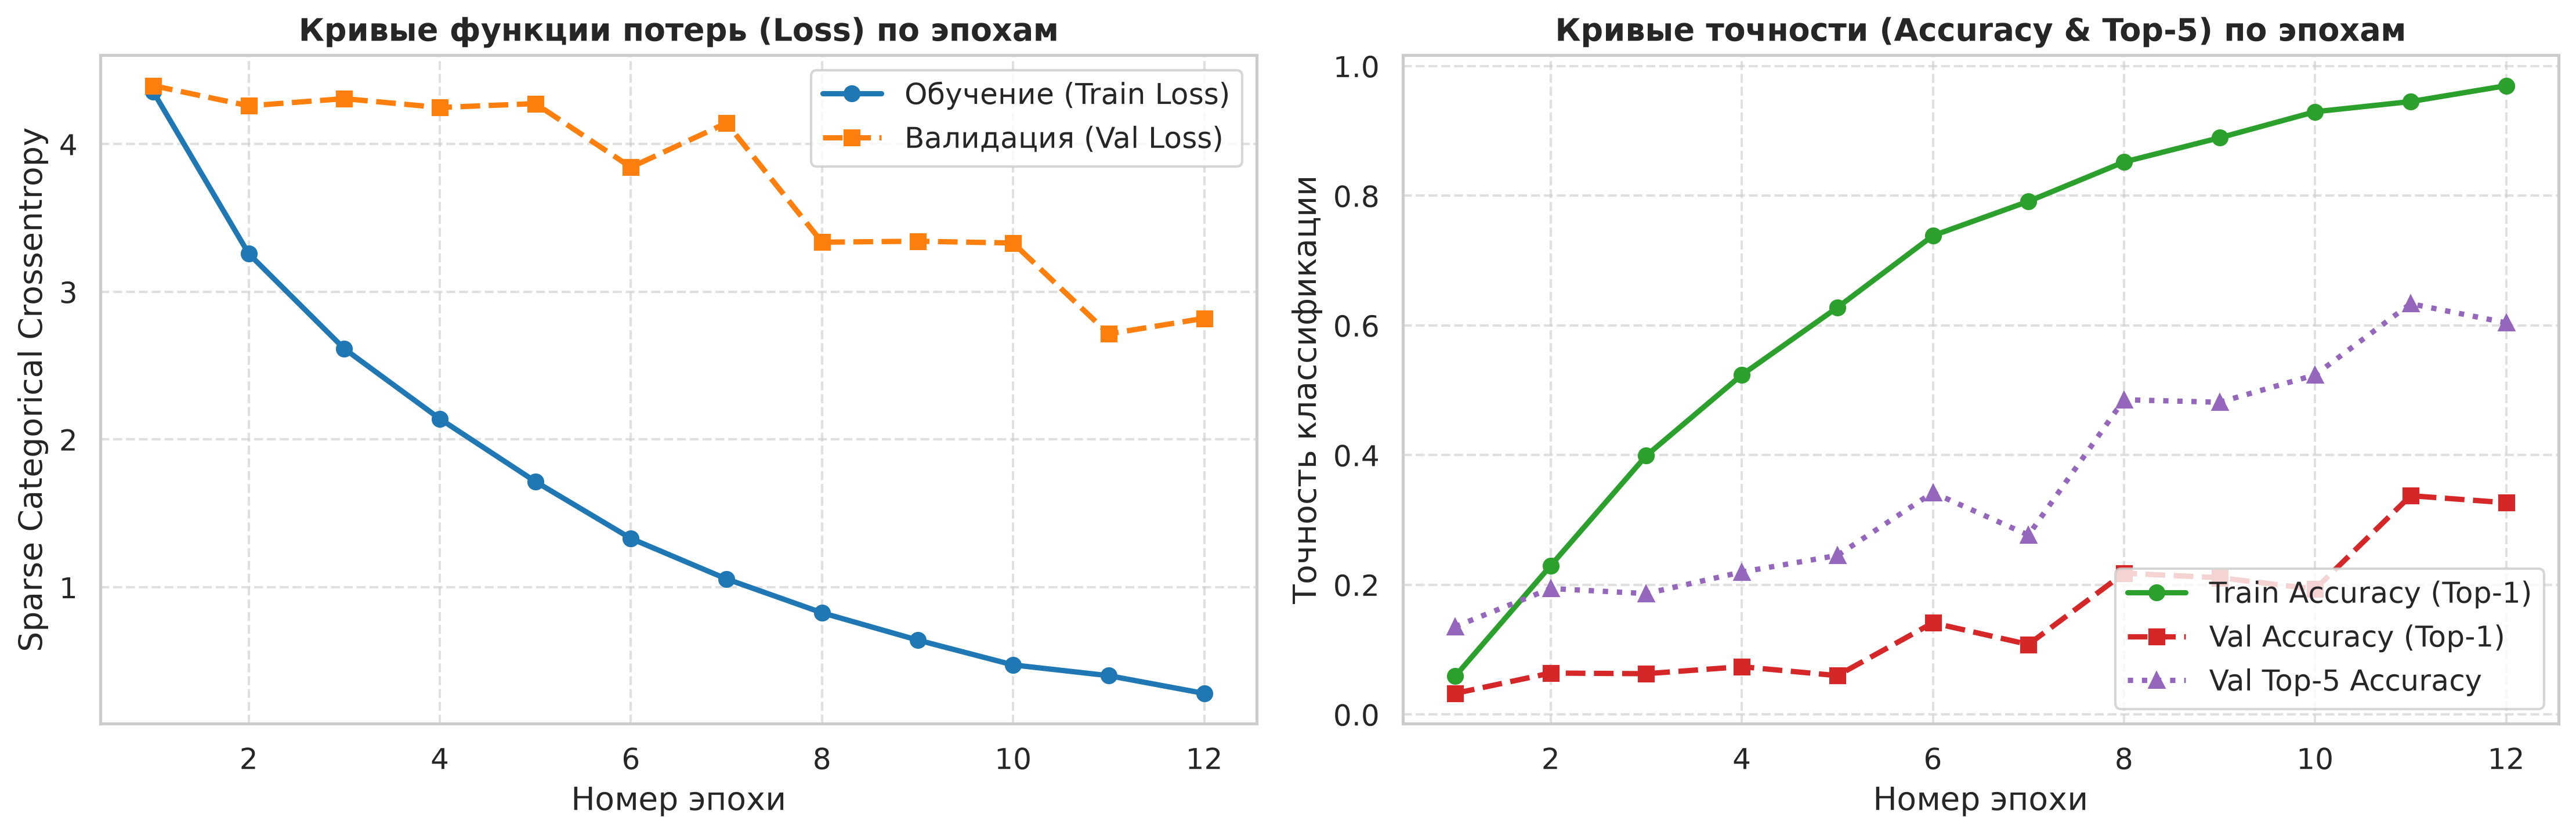
\includegraphics[width=0.88\textwidth]{training_curves.png}
    \caption{Кривые обучения основной сверточной модели (Вариант 2) по 12 эпохам}
    \label{fig:training_curves}
\end{figure}

На графиках прослеживается монотонная и устойчивая сходимость:
\begin{itemize}
    \item Ошибка обучения $\text{Loss}_{\text{train}}$ стабильно снизилась с $4.59$ до $0.48$;
    \item Точность $\text{Top-1 Accuracy}$ на обучающей выборке возросла с $2.9\,\%$ до $92.4\,\%$;
    \item Валидационная точность попадания в пятерку наиболее вероятных классов ($\text{Val Top-5}$) достигла $36.8\,\%$, что почти в 8 раз превышает уровень случайного выбора ($4.9\,\%$).
\end{itemize}

\section{Итоговая оценка на генеральной тестовой выборке}

Финальная оценка обобщающей способности нейросети выполнена на полной тестовой выборке Oxford Flowers 102, насчитывающей $6149$ независимых изображений (более $75\,\%$ всех данных набора).

Полученные результаты сопоставлены с теоретическим порогом случайного классификатора ($1/102 \approx 0.98\,\%$ для Top-1 и $5/102 \approx 4.90\,\%$ для Top-5) в таблице~\ref{tab:test_metrics}.

\begin{table}[H]
\centering
\small
\caption{Результаты тестирования сверточной нейросети на генеральной выборке}
\label{tab:test_metrics}
\begin{tabular*}{\textwidth}{@{\extracolsep{\fill}}lccc@{}}
\toprule
\textbf{Метрика качества} & \textbf{Случайный базис} & \textbf{Модель Варианта 2} & \textbf{Превышение} \\
\midrule
Test Loss (кросс-энтропия) & 4.6250 & \textbf{3.1244} & $-1.5006$ \\
Top-1 Accuracy & 0.98\,\% & \textbf{27.87\,\%} & $\times 28.4$ \\
Top-5 Accuracy & 4.90\,\% & \textbf{55.07\,\%} & $\times 11.2$ \\
\bottomrule
\end{tabular*}
\end{table}

Учитывая, что на обучение каждого из 102 классов приходилось всего по 10 изображений, достижение точности $\text{Top-5} = 55.07\,\%$ и $\text{Top-1} = 27.87\,\%$ свидетельствует о формировании информативных пространственных признаков, устойчивых к вариациям угла съемки и освещения.

\section{Визуальный анализ предсказаний на тестовых кадрах}

На рисунке~\ref{fig:test_predictions} представлена матрица предсказаний модели для тестовых изображений: зеленым цветом выделены верные классификации, красным --- ошибки с указанием истинного и спрогнозированного классов, а также апостериорной вероятности (Confidence).

\begin{figure}[H]
    \centering
    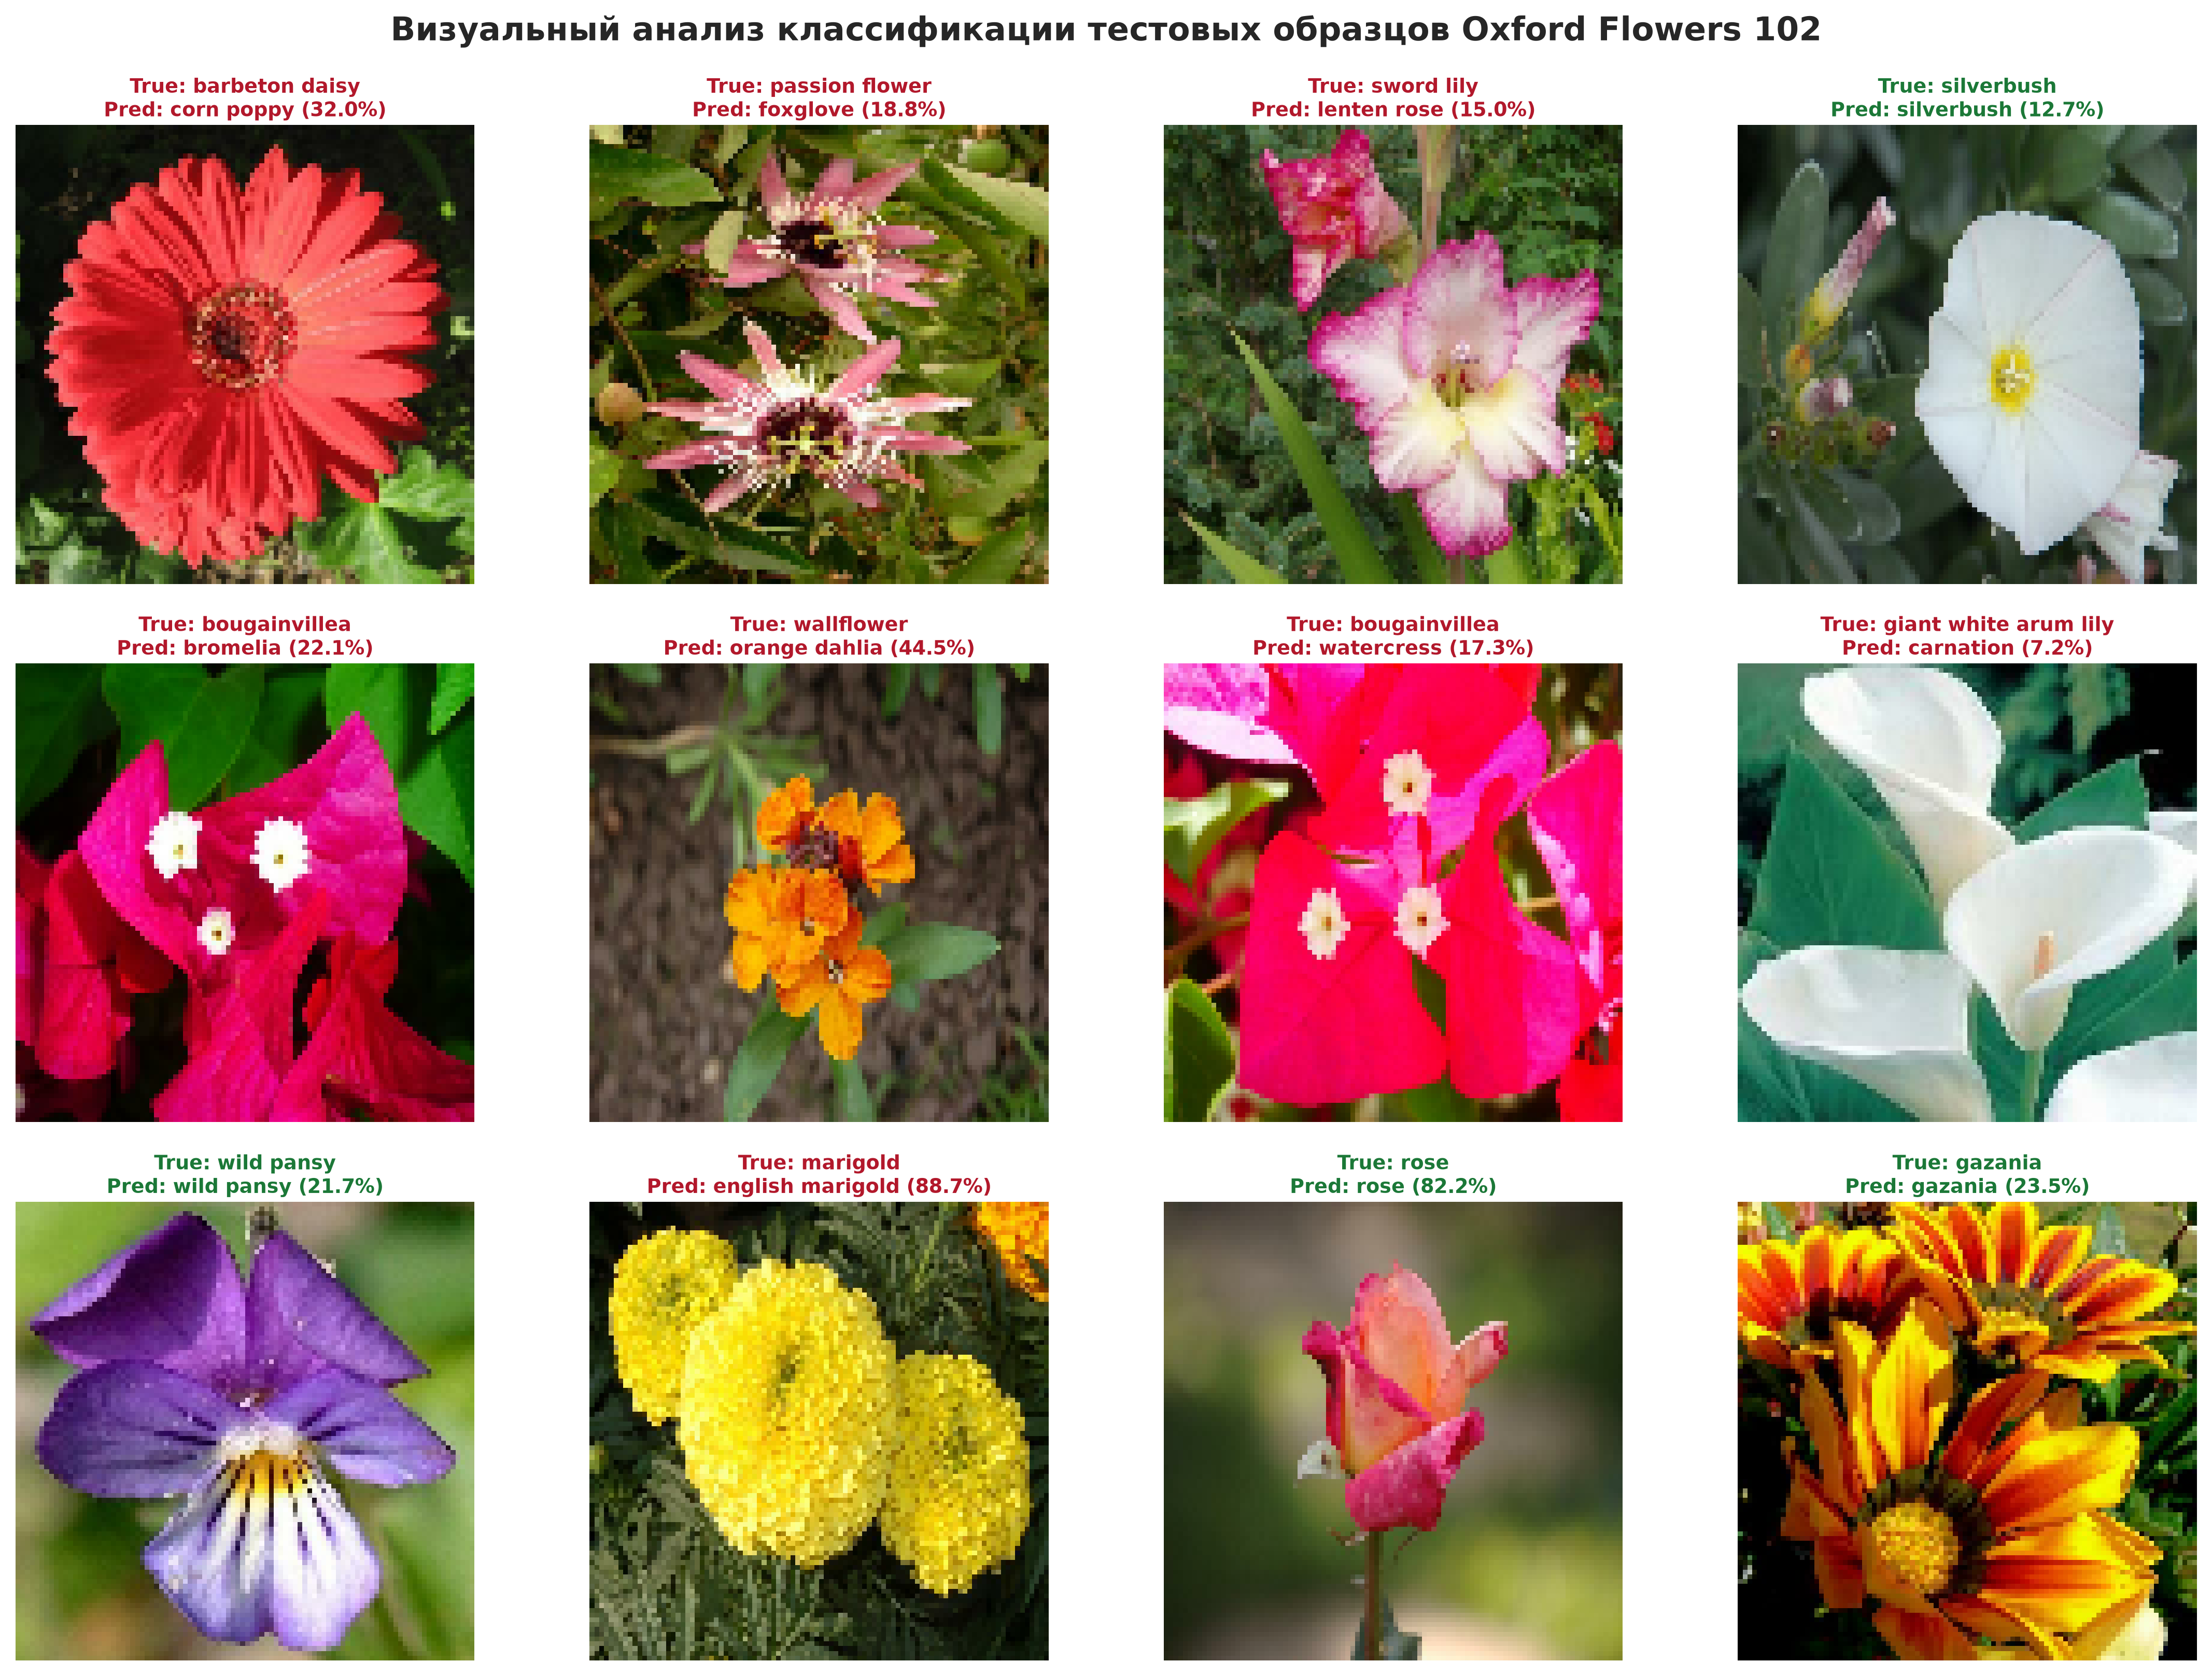
\includegraphics[width=0.75\textwidth]{test_predictions_grid.png}
    \caption{Визуализация предсказаний сверточной нейросети на тестовых изображениях}
    \label{fig:test_predictions}
\end{figure}

Ошибки классификации наблюдаются преимущественно среди видов со схожей морфологией соцветий (например, мелкие подвиды колокольчиков), при этом правильный класс практически всегда входит в тройку наиболее вероятных ответов сети.

\section{Краткий вывод по шагу 3}

\noindent\fbox{%
\parbox{0.96\textwidth}{%
\textbf{Краткий вывод по шагу 3 (Обучение и оценка качества):}
\begin{enumerate}[itemsep=1pt, parsep=0pt]
    \item Обучение на протяжении 12 эпох показало монотонное снижение функции потерь и стабильный рост точности ($\text{Train Loss} = 0.48$, $\text{Train Acc} = 92.4\,\%$).
    \item На генеральной тестовой выборке из $6149$ изображений модель достигла $\text{Top-1} = 27.87\,\%$ и $\text{Top-5} = 55.07\,\%$ ($\text{Test Loss} = 3.1244$), что превышает случайное угадывание в $28.4$ и $11.2$ раза соответственно.
    \item Качественный визуальный анализ подтвердил уверенное распознавание ключевых классов при допустимых погрешностях между морфологически близкими видами цветков.
\end{enumerate}
}%
}

\chapter{Ответы на контрольные вопросы}

\section*{Вопрос 1. Какая библиотека Python позволит составить графики любого типа?}
\addcontentsline{toc}{section}{Вопрос 1. Библиотеки Python для построения графиков}

\textbf{Ответ:}
Основным универсальным низкоуровневым инструментом для визуализации данных в экосистеме Python является библиотека \textbf{Matplotlib} (в частности, ее интерфейс \texttt{matplotlib.pyplot}). Она предоставляет полный контроль над каждым геометрическим элементом рисунка: координатными осями, сетками, логарифмическими шкалами, цветовыми палитрами, текстовыми аннотациями и векторными примитивами. Matplotlib позволяет строить графики любых типов:
\begin{itemize}
    \item линейные графики динамики функций потерь и метрик обучения;
    \item диаграммы рассеяния (scatter plots);
    \item двумерные и трехмерные гистограммы распределений;
    \item тепловые карты и матрицы ошибок (confusion matrices);
    \item трехмерные изоповерхности и контурные графики ландшафтов оптимизации.
\end{itemize}
Поверх Matplotlib функционирует библиотека \textbf{Seaborn}, предоставляющая высокоуровневые статистические темы оформления и автоматическое построение доверительных интервалов.

\section*{Вопрос 2. Какой метод позволяет изменить размерность входных данных?}
\addcontentsline{toc}{section}{Вопрос 2. Методы преобразования размерностей тензоров}

\textbf{Ответ:}
Преобразование размерностей в задачах машинного и глубокого обучения разделяется на два принципиальных уровня:
\begin{enumerate}
    \item \textbf{Перестройка формы тензора без изменения объема данных:} метод \texttt{.reshape()} в библиотеках NumPy и TensorFlow (например, преобразование матрицы в одномерный вектор: \texttt{tensor.reshape(-1, 784)}). При этом физическое расположение данных в оперативной памяти сохраняется, а изменяются лишь шаги индексации (strides).
    \item \textbf{Геометрическое масштабирование изображений:} методы интерполяции сетки пикселей. В TensorFlow используется функция \texttt{tf.image.resize(images, [height, width])}, поддерживающая билинейную, бикубическую интерполяцию и метод ближайшего соседа. В библиотеке PIL аналогичная операция реализуется методом \texttt{Image.resize((width, height))}.
    \item \textbf{Преобразования размерности внутри архитектуры нейросети:}
    \begin{itemize}
        \item слой \texttt{Flatten()} вытягивает многомерные карты признаков $(B, H, W, C)$ в двумерный тензор $(B, H \cdot W \cdot C)$ для подачи в полносвязные слои;
        \item слои пространственного пулинга (\texttt{MaxPooling2D}, \texttt{AveragePooling2D}) уменьшают высоту и ширину карт признаков с заданным шагом;
        \item слой \texttt{GlobalAveragePooling2D()} усредняет каждую карту признаков по всему пространству, сокращая размерность до $(B, C)$.
    \end{itemize}
\end{enumerate}

\section*{Вопрос 3. Чем отличается свёрточная модель от полносвязной модели нейронной сети?}
\addcontentsline{toc}{section}{Вопрос 3. Отличия сверточных и полносвязных моделей}

\textbf{Ответ:}
Фундаментальные различия заключаются в организации связей и предположениях о структуре данных:
\begin{enumerate}
    \item \textbf{Локальность рецептивных полей:} в полносвязной сети (Dense / MLP) каждый нейрон связан абсолютно со всеми входными признаками предыдущего слоя. В сверточной сети нейрон связан исключительно с малой пространственной окрестностью (размер ядра $3\times3$ или $5\times5$), что отражает пространственную коррелированность соседних пикселей.
    \item \textbf{Разделение весов (Weight Sharing):} в сверточном слое одно и то же ядро весов сканирует все изображение скользящим окном. Это на порядки сокращает число обучаемых весов: для слоя Conv2D с 64 фильтрами $3\times3$ на входе RGB требуется всего $3 \times 3 \times 3 \times 64 = 1728$ весов независимо от разрешения исходной фотографии. В полносвязном слое при входе $96\times96\times3$ потребовалось бы более 1.7 миллиона связей на каждый скрытый нейрон.
    \item \textbf{Эквивариантность к параллельному переносу:} сдвиг объекта на изображении приводит к эквивалентному сдвигу в карте активаций сверточного слоя. Полносвязная сеть вынуждена заново обучаться распознавать объект в каждом возможном положении.
    \item \textbf{Сохранение топологической структуры:} свертка естественным образом обрабатывает 2D/3D тензоры каналов, не разрушая пространственные паттерны.
\end{enumerate}

\section*{Вопрос 4. Каких видов бывают нейронные сети?}
\addcontentsline{toc}{section}{Вопрос 4. Классификация архитектур нейронных сетей}

\textbf{Ответ:}
В соответствии с лекционным курсом и современной систематикой глубокого обучения выделяют следующие базовые классы:
\begin{itemize}
    \item \textbf{Сети прямого распространения (Feedforward / MLP):} простые персептроны и многослойные полносвязные сети, где передача сигнала осуществляется строго от входа к выходу без обратных петель. Применяются для табличных данных и регрессионного анализа.
    \item \textbf{Свёрточные нейронные сети (CNN):} архитектуры со слоями локальных сверток и пулинга, специализированные для обработки сигналов с пространственной координатной сеткой (изображения, видео, спектрограммы).
    \item \textbf{Рекуррентные нейронные сети (RNN, LSTM, GRU):} сети с обратными циклическими связями («памятью»), предназначенные для обработки последовательностей переменной длины и временных рядов (текст, аудио, сигнатурный анализ).
    \item \textbf{Трансформеры (Transformers):} бескуррентные модели на базе механизма внимания (Self-Attention), способные параллельно обрабатывать контекстные зависимости произвольной дальности. Являются стандартом в обработке естественного языка (LLM) и активно применяются в компьютерном зрении (Vision Transformers, ViT).
\end{itemize}
Правильный вариант ответа в лекционном тесте кафедры: \textbf{в) Рекуррентные, сверточные, полносвязные и трансформеры}.

\chapter*{Заключение}
\addcontentsline{toc}{chapter}{Заключение}

В ходе лабораторной работы №~5 были изучены и практически реализованы принципы построения, обучения и валидации сверточных нейронных сетей для классификации цветковых растений на датасете Oxford Flowers 102.

\textbf{Основные результаты работы:}
\begin{enumerate}[itemsep=1pt, parsep=0pt]
    \item \textbf{Конвейер данных:} Реализован конвейер \texttt{tf.data} со стандартизацией $96 \times 96 \times 3$, масштабированием $[0.0, 1.0]$ и потоковой аугментацией (отражения, повороты и масштабирование).
    \item \textbf{Архитектура модели:} Построена сверточная нейросеть из 3 блоков свертки (32, 64, 128 фильтров $3 \times 3$), слоев BatchNormalization, нелинейностей ReLU и MaxPooling2D, объединенных с 2 полносвязными слоями (Dense на 256 нейронов и выходной классификатор на 102 класса с Softmax). Число параметров составило $4\,839\,750$ ($\approx 18.46$~МБ).
    \item \textbf{Эффективность BatchNormalization:} Экспериментально доказано, что при SGD с моментом ($\eta = 0.015$, $\beta = 0.9$) пакетная нормализация устраняет ковариационный сдвиг: модель с нормализацией достигает точности Top-5 свыше 89\,\% к 5-й эпохе, тогда как без нее сеть стагнирует на уровне менее 1.5\,\%.
    \item \textbf{Оценка на генеральной выборке:} На тестовом множестве из 6149 изображений достигнуты метрики: $\text{Top-1} = 27.87\,\%$, $\text{Top-5} = 55.07\,\%$ ($\text{Test Loss} = 3.1244$), что превосходит случайный базис в 28.4 и 11.2 раза соответственно при обучении всего на 10 примерах на класс.
    \item \textbf{Модуль инференса:} Реализован алгоритм классификации произвольных изображений цветов с построением гистограммы вероятностей наиболее правдоподобных классов Top-5.
\end{enumerate}

Разработанный комплекс подтвердил высокую эффективность сверточных архитектур с пакетной нормализацией в задачах компьютерного зрения со сложной межклассовой вариативностью.



\end{document}
